\chapter{Direct aggregation of sea level from mesoscale forecasts and tide predictions}
\label{chp:aggregate}
%-----------------------
\begin{quote}
{\small
Originally published as: \texttt{
Taylor, A. J. and Brassington, G. Sea Level Forecasts Aggregated from Established Operational Systems. Journal of Marine Science and Engineering 5, 33 (2017)}.

A system for providing routine seven-day forecasts of sea level observable at tide gauge locations is described and evaluated.
Forecast time series are aggregated from well-established operational systems of the Australian Bureau of Meteorology; although following some adjustments these systems are only quasi-complimentary.
Target applications are routine coastal decision processes under non-extreme conditions.
The configuration aims to be relatively robust to operational realities such as version upgrades, data gaps and metadata ambiguities.
Forecast skill is evaluated against hourly tide gauge observations.  
Characteristics of the bias correction term are demonstrated to be primarily static in time, with time varying signals showing regional coherence.
This simple approach to exploiting existing complex systems can offer valuable levels of skill at a range of Australian locations.
The prospect of interpolation between observation sites and exploitation of lagged-ensemble uncertainty estimates could be meaningfully pursued. 
Skill characteristics define a benchmark against which new operational sea level forecasting systems can be measured. 
More generally, an aggregation approach may prove to be optimal for routine sea level forecast services given the physically inhomogeneous processes involved and ability to incorporate ongoing improvements and extensions of source systems.
}
\end{quote}

\section{Chapter introduction}
\subsection{Routine sea level and operations}

% sea level is relevant
Of the activities that now constitute `operational oceanography' \citep{Bell:2009uv}, sea level forecasting possibly has the most historical baggage as well as the most widespread application.
Day-to-day routine decisions are based on quantitative expectations of still water level \citep{Pugh:2014di} at the coast.  
For example in marina and managed estuary operations, maritime under keel clearance systems and coastal works scheduling. 
Such routine decisions do not involve sea level extremes such as during tropical cyclones and tsunamis---and rare extremes are not addressed here. 
The focus of this paper is routine sea level forecasting that includes the superposition of relatively moderate phenomena.
Figure \ref{fig:fc_eg} is an~illustrative example of how such forecast guidance can be presented. 


%% operational is special
%All models are wrong, but some are useful \citep{Box:1979wz}\hl{and}
%Please check this change.
% some are operational.
%All models are wrong, but some are useful \citep{Box:1979wz} ...and some are operational.    
All models are wrong, but some are useful \citep{Box:1979wz}; and some are operational.        % FINAL PROOF: author intention was a twist on the Box cliche.   Originally had ellipsis but semicolon fine too.  (A,B ...C) or (A,B;C) 
Forecast systems that enjoy ongoing and reliable operational support are of particular relevance to users.
Existing operational systems also set a relevant benchmark for the justification of the development of new~systems.  

\begin{figure}[!hbt] \centering
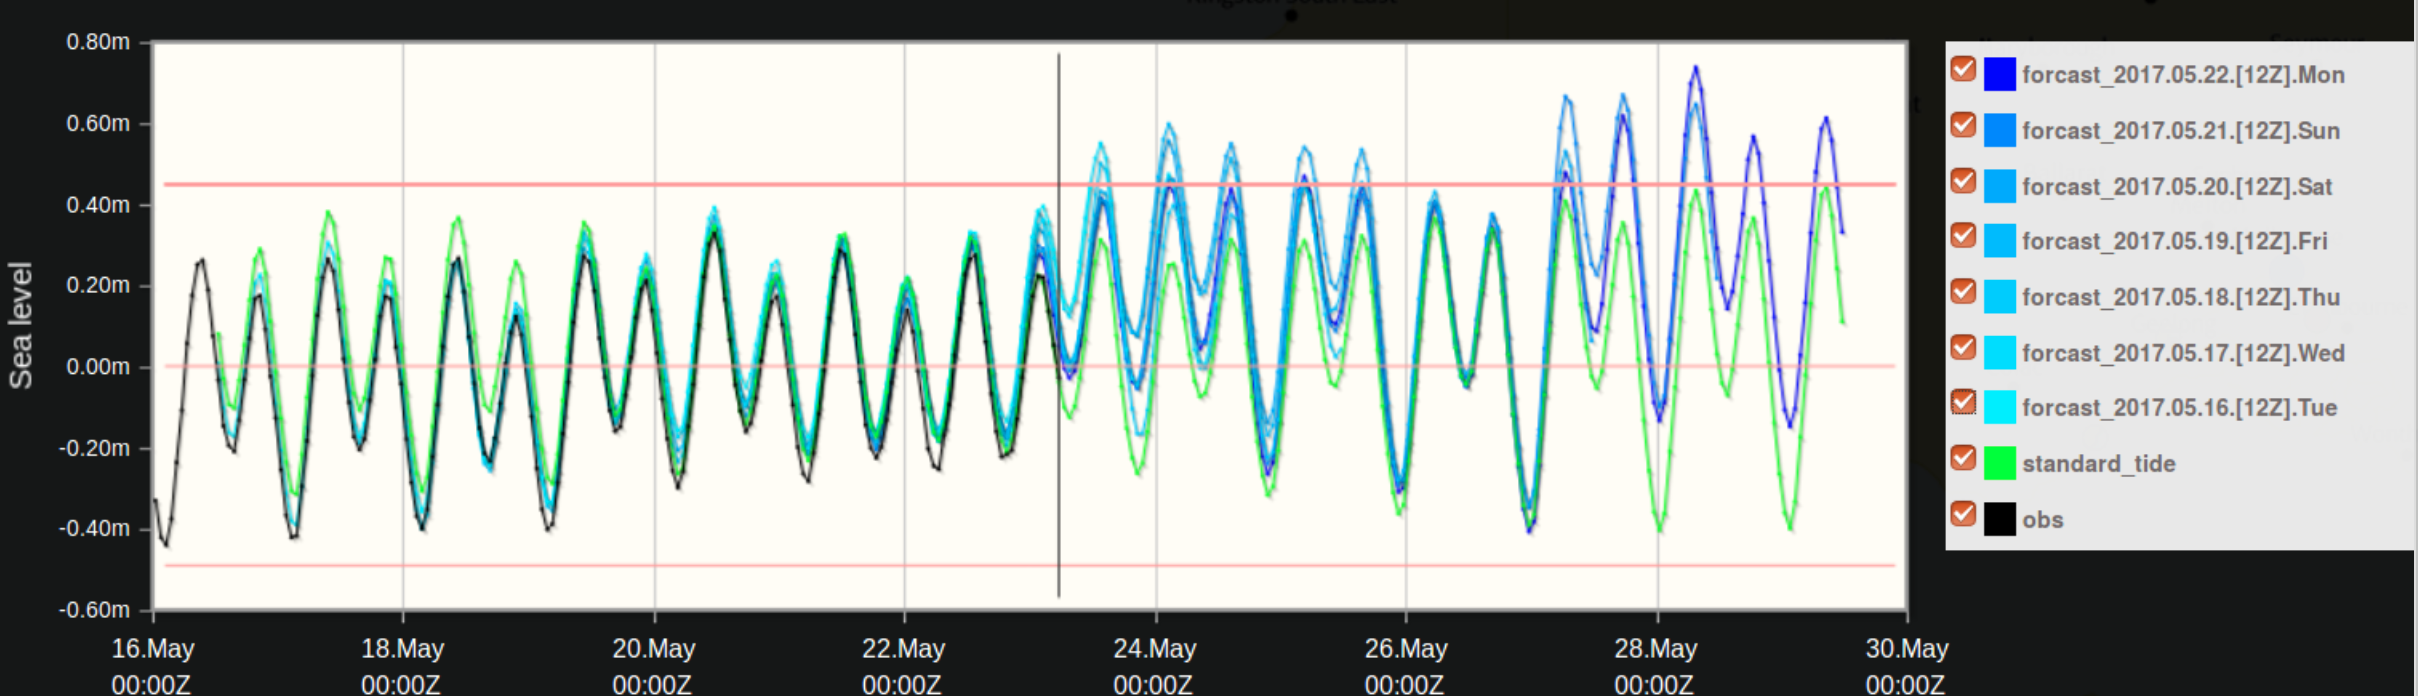
\includegraphics[width=1\textwidth]{figures/plots/forecast_eg.png}
\caption{Sea level forecast display.}{Illustrative sea level forecast for St Kilda at Melbourne, Australia.  Sequential 7-day forecasts are shown overlaid in shades of blue.  Observed sea level is shown in black and standard tide prediction in green.  Red horizontal lines indicate conventional tidal planes LAT, MSL and HAT.  Some spread is apparent between forecast updates.  Sea level is not especially extreme, but is forecast to cross the reference HAT in coming days.}
\label{fig:fc_eg}
\end{figure}   


%% sea level and different models 
Observed sea level is a manifestation of diverse physical processes and scales; some local in nature, but many involving signal propagation \citep{Melet:2016dd}.
The balance of contributions varies across the vast geographic range of the Australian coastline \citep{Haigh:2013bn,Haigh:2013he,Woodham:2013cl,Ridgway:2004kb,Church:1986tl,Allen:2009tf}.

% evolution of targeted physical models
Specialised forecasting approaches have evolved to target different scales and subcomponents of sea level \citep{Cartwright:2000tt,Petersen:2012kp}.
A variety of systems relevant to sea level are now in side-by-side, but isolated, operation in organisations such as the Australian Bureau of Meteorology (BoM). 
These capabilities include in situ and remote observations, conventional tide predictions, wave spectra forecasts, river run-off routing and tsunami models. 
More recently, data assimilating primitive equation ocean models~\citep{Schiller:2011dia} have come into operational centres via a path broadly analogous to the development of numerical weather prediction \citep{Harper:kb}. 

Inevitably the foundations of operational global forecasts are being leveraged for localised downscaled dynamic operational ocean models: e.g., \citep{Paramygin:2017dx,Yang:2016ep,Wei:2014ex,Peng:2014kq}.

However, spatial and temporal coverage is non universal; and relevance to everyday decision makers is not necessarily a direct function of increased model resolution.  


%% harmonic tides are special - data driven
\subsection{Conventional tides}
\label{sec:tide_intro}

Conventional tide predictions are a remarkably successful data-driven forecast product that provides an omni-present reference for coastal activities.
By design these make no account for aperiodic phenomena. 
Production involves time series statistics based on historical records of observations at each forecast site.
Importantly, the observations need not be recently collected; let alone delivered in real time.

Tidal techniques exploit the significance of periodic sea level variations observed to be coherent with the `astronomical tide generating forces (ATGF)' \citep{Hendershott:1981ub}.     
Many variations exist for implementing this general approach (e.g., \citep{Foreman:2009bg,Groves:1975ky,LEFFLER:2009ej,Smith:1997ut} ). 
Useful sea level predictions can thereby be produced many years into the future.  
Tidal methods based on a harmonic decomposition of the ATGF have long been typical of bodies promulgating `official' tidal products; including BoM.
Official tidal products have come to have a special status; for instance, statistical properties of tidal predictions define elevation references for mapping and legal applications \citep{PCTMSL-sp9}.

% ...periodic but not astro 
The ongoing value of standard tidal predictions reflects the fact that periodic signals generally dominate routine coastal still water levels.
However, the physical drivers of sea level represented in tidal predictions need not be gravitational at all.
Treatment of non-gravitational signals is a practical consideration in tidal analysis procedures; notably for the long-period constituents Sa and Ssa (\citep[]{Parker:2007wq} Sect. 3.7) but also at shorter timescales such as constituent S1 \citep{Ray:2004ts}.
The extent to which conventional harmonic tidal predictions are `physics free' actually allows for a pragmatic flexibility to represent almost all of the everyday rise and fall of coastal sea level at a place.

Even when relatively high resolution dynamic tidal models are available, the standard tide predictions at a place are commonly considered a superior estimate of routine sea level \citep{Horsburgh:2008gw,Egbert:1996vr}.


% real time insitu obs
\subsection{Real time observations}
Conventional tide methods have had such a long time to become deeply embedded \citep{Cartwright:2000tt} thanks to the ability to produce useful forecasts via access to observations only in a much lagged batch mode.  
In contrast, tide gauge observations are increasingly communicated in near real time to operational centres and general users. 
BoM operates its own network of tide gauges \citep{Greenslade:2012um} but the majority of available observations are shared by partner or `3rd party' organisations. 
Gathering observations from diverse organisations is valuable but can raise issues with data quality and metadata management.

Despite the nominal co-location of real-time tide gauge observations and various forecasting systems, presentation of useful verifiable guidance has been found to be surprisingly elusive.     

While more real time observations in principle opens opportunities for assimilation into dynamic models or various `trained' forecast systems \citep{Horsburgh:2011th}, such use can place much weight on the reliability and quality control of live data streams; a non-trivial concern over large regions and multiple agencies \citep{Mourre:2006hz}.


%----------------------------------------------------------------------------------------------------------------------------
\section{Forecast system description}
\subsection{Motivation}
This work is founded on the operational maturity of a global ocean forecast system (OceanMAPS) within an agency that also provides weather, tide and river forecasts.
The demonstration of limited non-tidal sea level forecast skill in earlier versions of OceanMAPS \citep{Taylor:2010ud} motivated investigation of potential practical applications. 
Liaison with forecasters and forecast-users lead to the current configuration; routine 7-day forecasts that can be directly evaluated against tide gauge observations.
A~secondary motivation was to establish a performance benchmark against which new sea level forecast capabilities can be evaluated. 

\subsection{Superposition}
\label{sec:concept}
% A generic 'one-size-fits-all' and parsimonious approach is taken.
The configuration is a linear superposition of time series derived from heterogeneous operational systems, schematically illustrated in Figure \ref{fig:aggSL} and Equation (\ref{eq:aggSL}).  
Although the superposition itself is linear, subsets of non-linear hydrodynamics are internally represented within the ocean circulation model  and the tidal harmonic fit respectively.

Component systems \textit{included} are listed here and described further below:
(1) Global ocean circulation forecasts---Section \ref{sec:dynamicmodels}, 
(2) Global numerical weather prediction---Section \ref{sec:dynamicmodels}, 
(3) adjusted harmonic tide predictions---Section \ref{sec:harmonics} and 
(4) observations-based bias correction---Section \ref{sec:bias}.

There are some notable \textit{exclusions} from the current configuration.
Spectral wave forecasts are available but not included on the basis that observation sites are located outside of surf zones (similar to  \citep{Tilburg:2004cg}).
River levels or outflow forecasts are not available in suitable form or coverage. In contrast, sea~level forecasts are an input into hydrological models \citep{Taylor:2011ud}.  

As the native time discretization of the input differ, each timeseries is projected onto a common 1-hourly format using an integral spline method.  
In the case of model inputs this is interpolation from 3-hourly averaged model outputs to 1-hourly.  
For observations the same method provides a~down-sampling from from 1-min or 15-min samples to 1-hourly averages.  
\begin{equation}
h(t) = \eta_{T}(t) - \eta_{HA}(t) + \eta_{SLA}(t) + \eta_{LIB}(t) + b(t0)
\label{eq:aggSL}
\end{equation}
where $h(t)$ is the aggregated sea level value at forecast time $t$.  
Signal components $\eta$ correspond to inputs in schematic Figure \ref{fig:aggSL} and subscripts $T$ and $HA$ indicate tide and harmonic adjustment respectively.    
Bias correction $b$ is a fixed value across each forecast.
\begin{figure}[!hbt] \centering
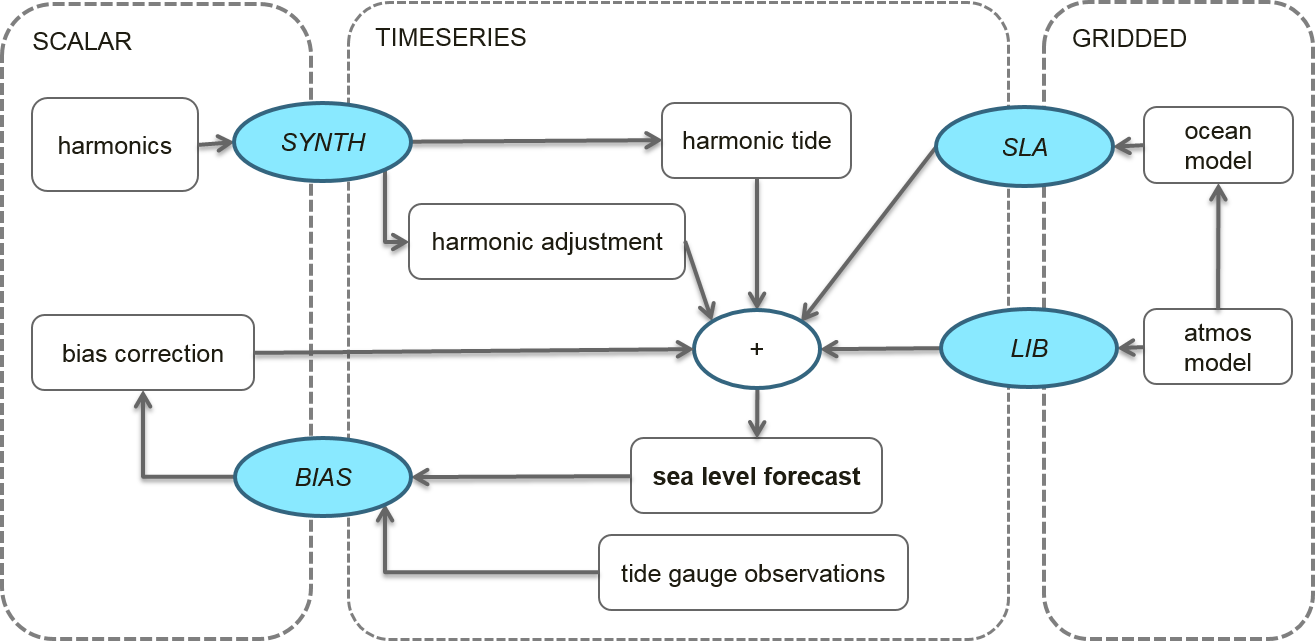
\includegraphics[width=1.0\textwidth]{figures/diagrams/aggSL_schematic_abstract.png}
\caption{Schematic configuration of aggregation system.}
{Source systems are heterogeneous but mapped onto time series that can be directly compared against 1-hourly observations.  (\textbf{SYNTH}) indicates tidal synthesis, (\textbf{SLA}) sea level anomaly from OceanMAPS, (\textbf{LIB}) local inverse barometer approximation based on atmospheric pressure forecast, (\textbf{BIAS}) non-causal filter bias correction scheme. }
\label{fig:aggSL}
\end{figure}   


% INPUT - oceanmaps and access
\subsection{Input: data assimilating primitive equation forecasts }
\label{sec:dynamicmodels}

Near-global ocean forecasts have been in operational production at the BoM now for 10 years via several versions of the Ocean Model, Analysis and Prediction System (`OceanMAPS')~\citep{Brassington:2007ut,NMOC:2007wq,BureauofMeterology:2011ta,Brassington:2012wm}.
The~dynamic ocean model component of OceanMAPS is based on the Modular Ocean Moel (`MOM')~\citep{Griffies:2008vh} configured with 0.1 $\times$ 0.1 degree regular structured horizontal resolution, hydrostatic free surface, z-level and split-implicit scheme; where the barotropic calculation is performed at a finer time stepping. 

Gravitation tidal forces are intentionally \textit{not} included in OceanMAPS.      


Land run-off fresh water fluxes are only roughly approximated with a climatological annual cycle. 
Australian rivers are typically dry for very long periods with intermittent flooding.   
The climatological river input is only included for maintaining global mass balance and has essentially no skill for Australian river outflow impacts on sea level.    


Initial conditions for the ocean state are constrained using an ensemble optimal interpolation data assimilation scheme \citep{Oke:2008wr} which ingests a large number and range of remote and in situ ocean observations. 
Importantly for sea level, tide gauge observations are \textit{not} assimilated and are independent.   
Satellite altimeter observations of sea level are assimilated, but not inshore of the shelf break; nominally cut off at the 200m isobath.


Atmospheric fluxes, excluding barometric pressure, are applied directly from the global numerical weather prediction (NWP) system ACCESS-G \citep{BureauofMeterology:C8IaJ2Qq}.
ACCESS-G is also based on a data assimilating primitive equation model.
It is not coupled with any ocean model beyond use of a persisted SST analysis boundary condition.
These flux fields are generated on a N512 gaussian grid with an indicative spatial resolution of~25 km. 
% (The NWP forecast fluxes extend for 10-days.)

OceanMAPS produces a new ocean state forecast each day for the next 7-days using a multi-cycle ensemble schedule \citep{GaryBBrassington:2013jw}.

As a result, 7-day forecasts of a sea level anomaly ($\eta_{SLA}$) quantity are reliably available each day.  
This data is output as 3-hourly averages.  
The quantity $\eta_{SLA}$ is not directly observable, but in the open water is observationally constrained by corrected altimeter observations.
$\eta_{SLA}$ is quantified relative to the model rest state, which nominally represents a geopotential surface like mean sea level.  

The regular spatial discretisation of OceanMAPS does not resolve features smaller than 10 km.   
In addition, some nominally larger embayments have also been intentionally excluded such as Port Phillip Bay in South Eastern Australia.
The Arakawa B-grid discretization imposes a numerical requirement to exclude 1-cell bays. 
A minimum depth of three z-levels equivalent to 15 m is also imposed.

The representation of the coast is illustrated in Figure \ref{fig:map_masks}.

In order to map the gridded $\eta_{SLA}$ field to a tide gauge location, a generic one-to-one `nearest coastal neighbour' algorithm is applied.
A manual exception for cell selection is applied to the Port Phillip case to ensure alignment with the single bay entrance. 
\begin{figure}[!hbt] \centering
    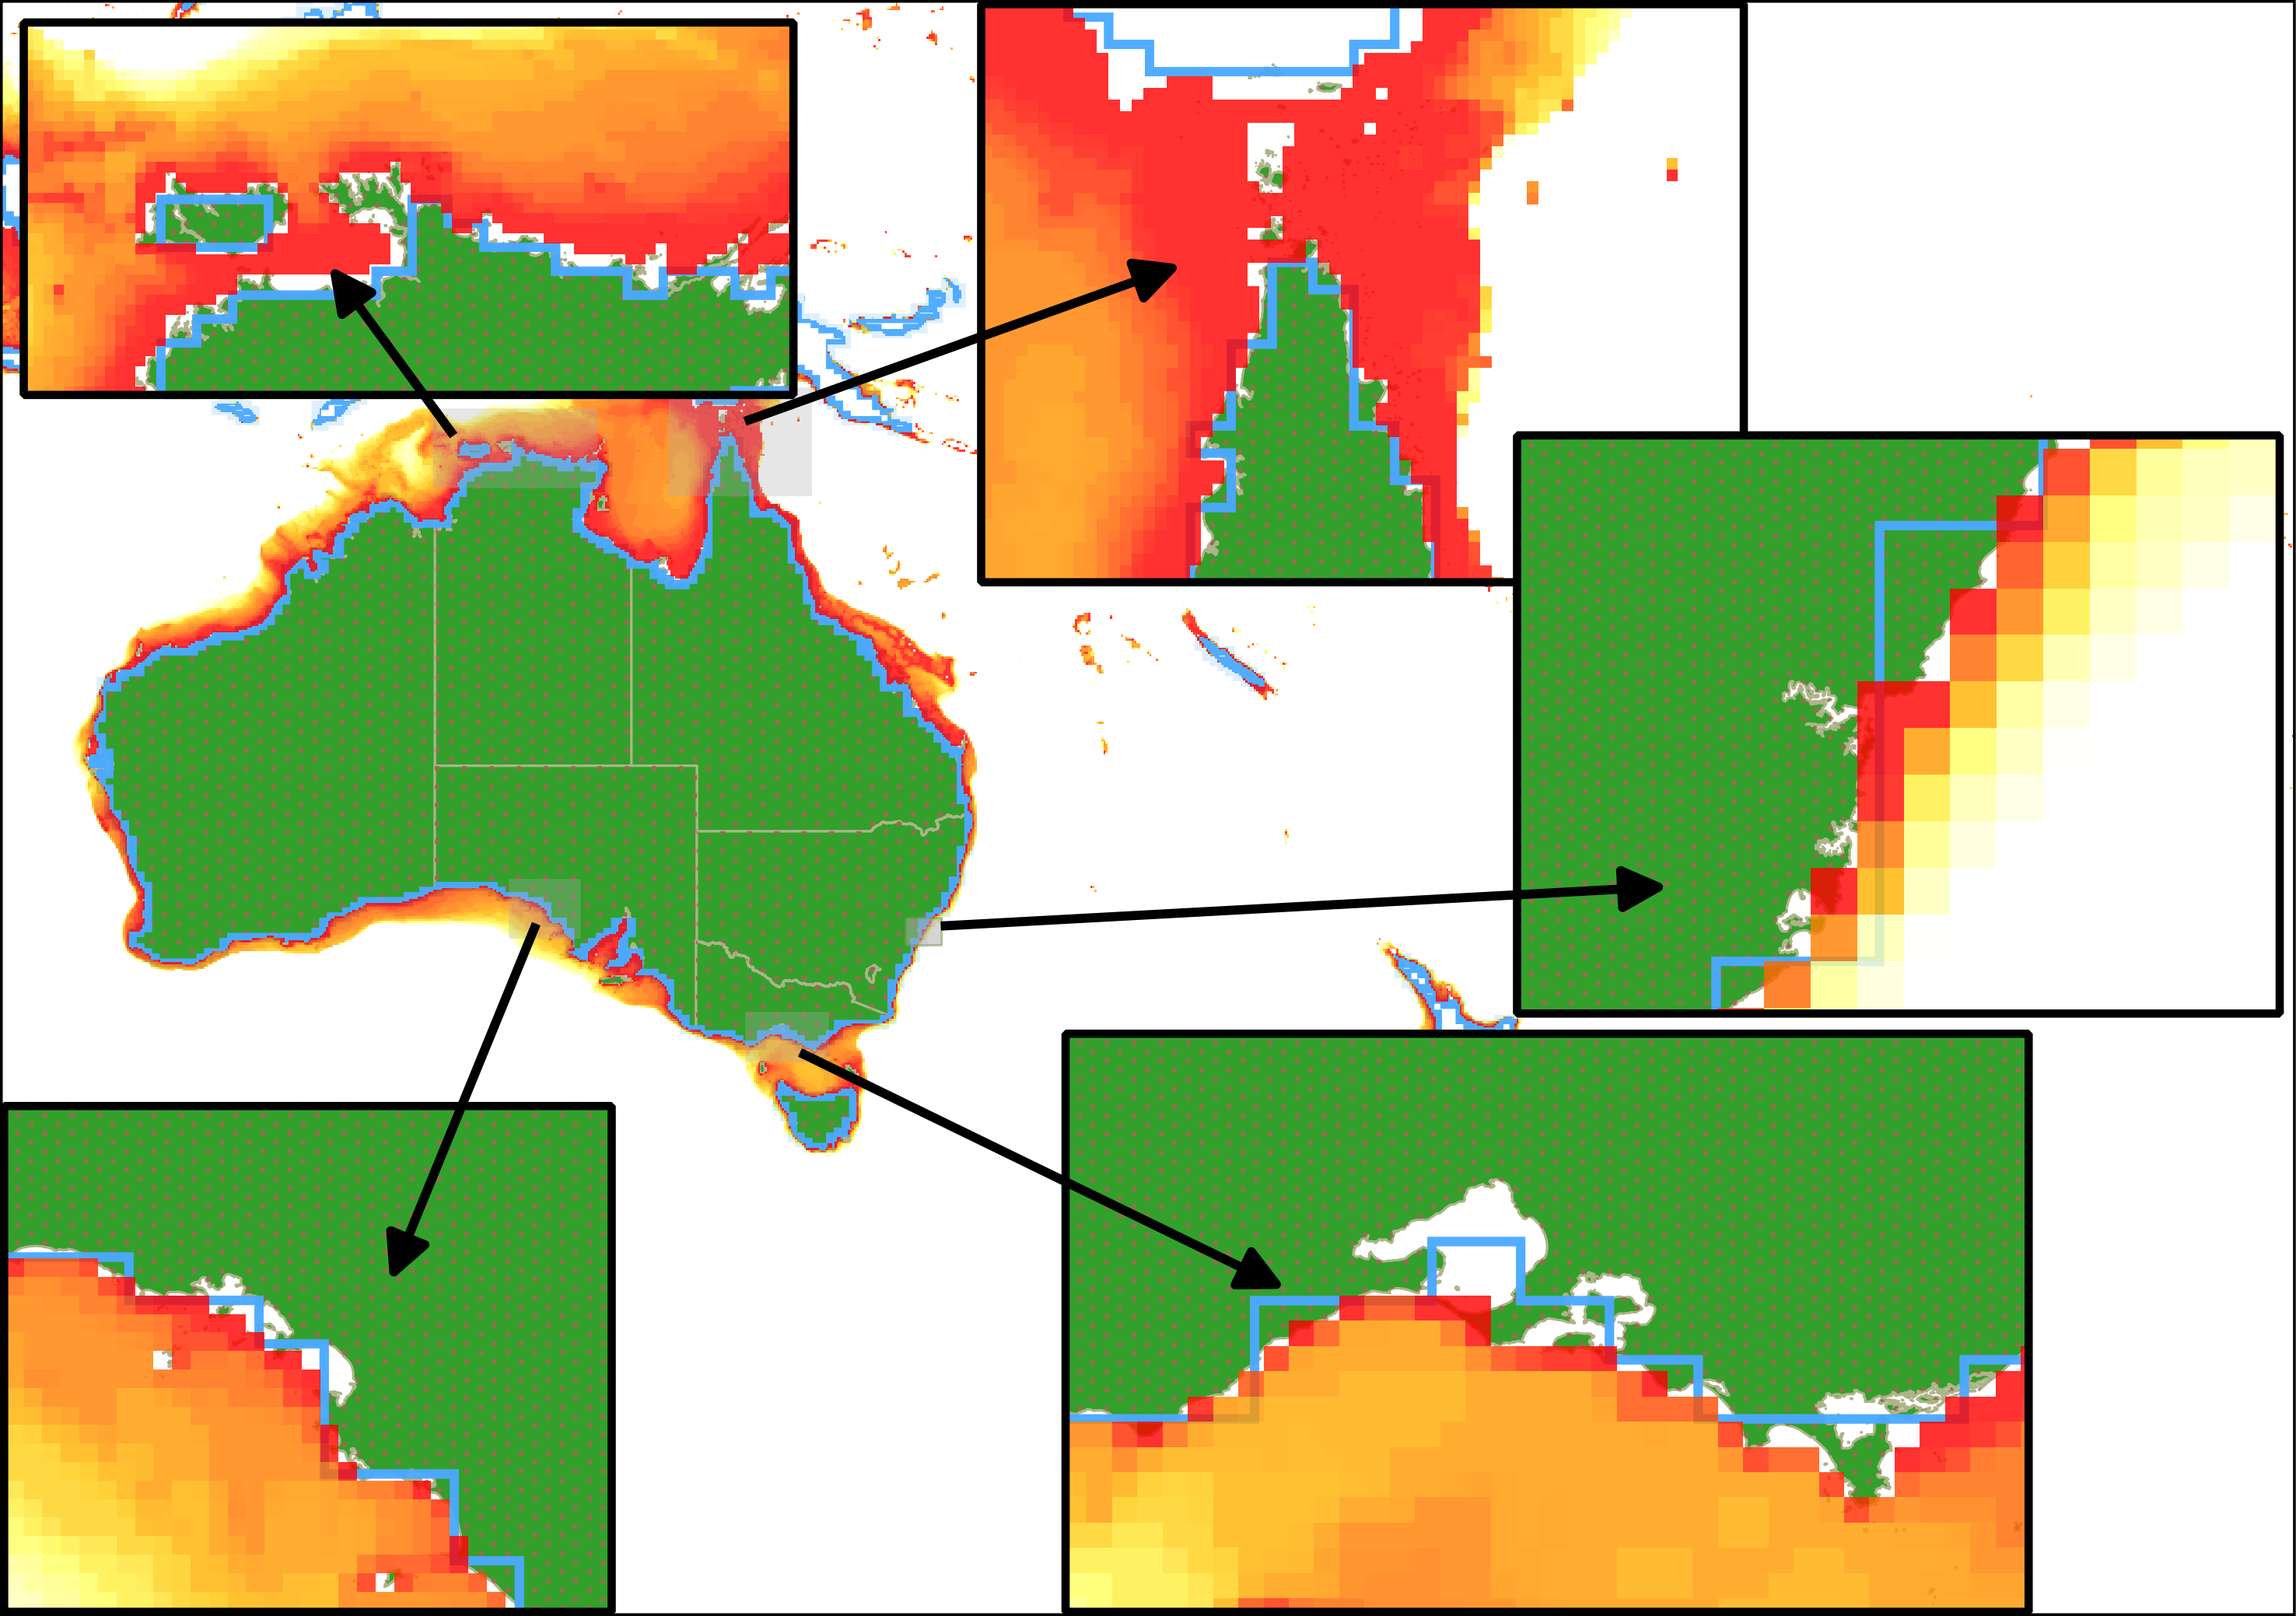
\includegraphics[width=1.0\textwidth]{figures/maps/omaps_masks.png}
    \caption{Coastal discretisation map and details.}
    {Red coloured grid cells indicate ocean model bathymetry the inner extent of which is the effective model coastline.  The thick blue line indicates the edge of the atmospheric model land/sea mask.  Most small scale features and embayments at tide gauge locations are only approximated at scales above~10 km in the ocean and~80 km in the atmosphere. }
    \label{fig:map_masks}
\end{figure}  


OceanMAPS does not represent the effect of atmospheric pressure forces on the ocean.
Subsequently, a local inverse barometer approximation is applied as per Equation (\ref{eq:lib}).
This formulation was chosen for being simple and robust, but is acknowledged as a compromise with regard to atmospheric representation and non-instantaneous ocean responses \citep{Mathers:2004bk}.
A fixed conventional reference pressure, rather than one derived from the NWP, was considered appropriate given the generic offset adjustment built into the bias correction scheme (Section \ref{sec:bias}).  
\begin{equation}
  \eta_{LIB} = \frac{ p_{NWP} - p_{ref} }{ \rho g }
  \label{eq:lib}
\end{equation}
where reference pressure is fixed at $p_{ref}$ = 101,325 Pa, and bulk sea water density is also kept fixed at 1027 $\text{kg}/\text{m}^3$.
Only a small subset of tide gauges are co-located with real-time barometer instruments.


\subsection{Input: tidal harmonics }
\label{sec:harmonics}
Officially promulgated tide predictions have a special relevance, as raised in Section \ref{sec:tide_intro}.
The~aggregation configuration intentionally aims to align with the BoM's existing tide tables. 

However, the heterogeneous nature of harmonic tide analysis and OceanMAPS configuration leads to a situation where the respective sea level signals are not cleanly complimentary.
In particular some of the sea level variation in the ocean model may be seen as `tidal', whereas some of the variation in the tidal harmonics may be seen as meteorological.   
In isolation, this spectral overlap is generally not problematic. 
However, linear superposition of the OceanMAPS $\eta_{SLA}$ with standard tides can lead to undesirable double-counting. 
This is most obvious at longer time scales in Northern Australia; where relatively powerful seasonal sea level changes have projected onto tidal harmonics.


A pragmatic approach is taken that aims to address both of these motivations; namely to align with other official tidal products and mitigate effects of spectral overlap.
The BoM's operationally supported tidal synthesis software is applied to two versions of tidal harmonics for each location:
\begin{itemize}
  \item full set of tidal harmonics: typically 114 constituents.
  \item subset assigned apriori to be primarily non-gravitational in expression: Sa, SSa, Mm, Msf and S1.
\end{itemize}

The subset time series is designated as a harmonic adjustment signal that is then subtracted within the superposition of signals. 


\subsection{Input: bias correction}
\label{sec:bias}
Near real-time observations are available at an increasing number of tide gauge locations, and~intuitively serve as a source of guidance to users.
Typical practice, though often not formalised, is~to~inspect recent tidal error (residual) evolution and project as a correction to tide tables into the near~future.

Operational availability of this source of information is exploited in a generic and untrained bias correction scheme. 
The bias term ($b$ in Equation (\ref{eq:aggSL})) is a constant added to each forecast.
The value of $b$ is derived as a weighted mean of recent errors between observed sea level and previous forecasts between 0--24 lead times.
The most recent value persists in the case of observation drop-outs and gaps.
Observations are pre-processed with a median spike filter to mitigate the impact of communications glitches and noise.
Weighting is tapered such that the influence of older error values decreases with time prior to the present and it is `causal' in the sense that no observations after the forecast base time have any influence.
The total window length of the filter spans 21 days.
Identical settings are applied to all locations.


The scheme aims to cover multiple needs.
Firstly, to address alignment of reference datums between sources. 
It is the temporal evolution of $\eta_{SLA}$ and $\eta_{LIB}$ that is expected to contain real information---not the absolute values.
Moreover, metadata ambiguity with regard to the reference datum of real-time observational streams (from 3rd parties) relative to tide prediction datums has proven to be a real issue.
Secondly, the correction serves as a crude data assimilation method to adjust the vertical offset of the forecast in light of long period error evolution. 

The actual behaviour of this term is discussed further in Section \ref{sec:bias_more}.

%----------------------------------------------------------------------------------------------------------------------------
\section{Evaluation}

Evaluation results are presented based on aggregate sea level forecasts produced in an operational mode at BoM between June 2016 to May 2017.

\subsection{Geographic overview}
Evaluation is restricted to a series of point locations.  These locations correspond to tide gauges from which real-time information was reported into the operational centre over the study period.  An overview map of these locations is shown in Figure \ref{fig:map_locations}.
The inconsistent coastal distance between locations is an outcome of human population distribution and inter-organisational arrangements.
It~is~foreseeable that the number of sites could expand significantly in the future.
\begin{figure}[!hbt] \centering
    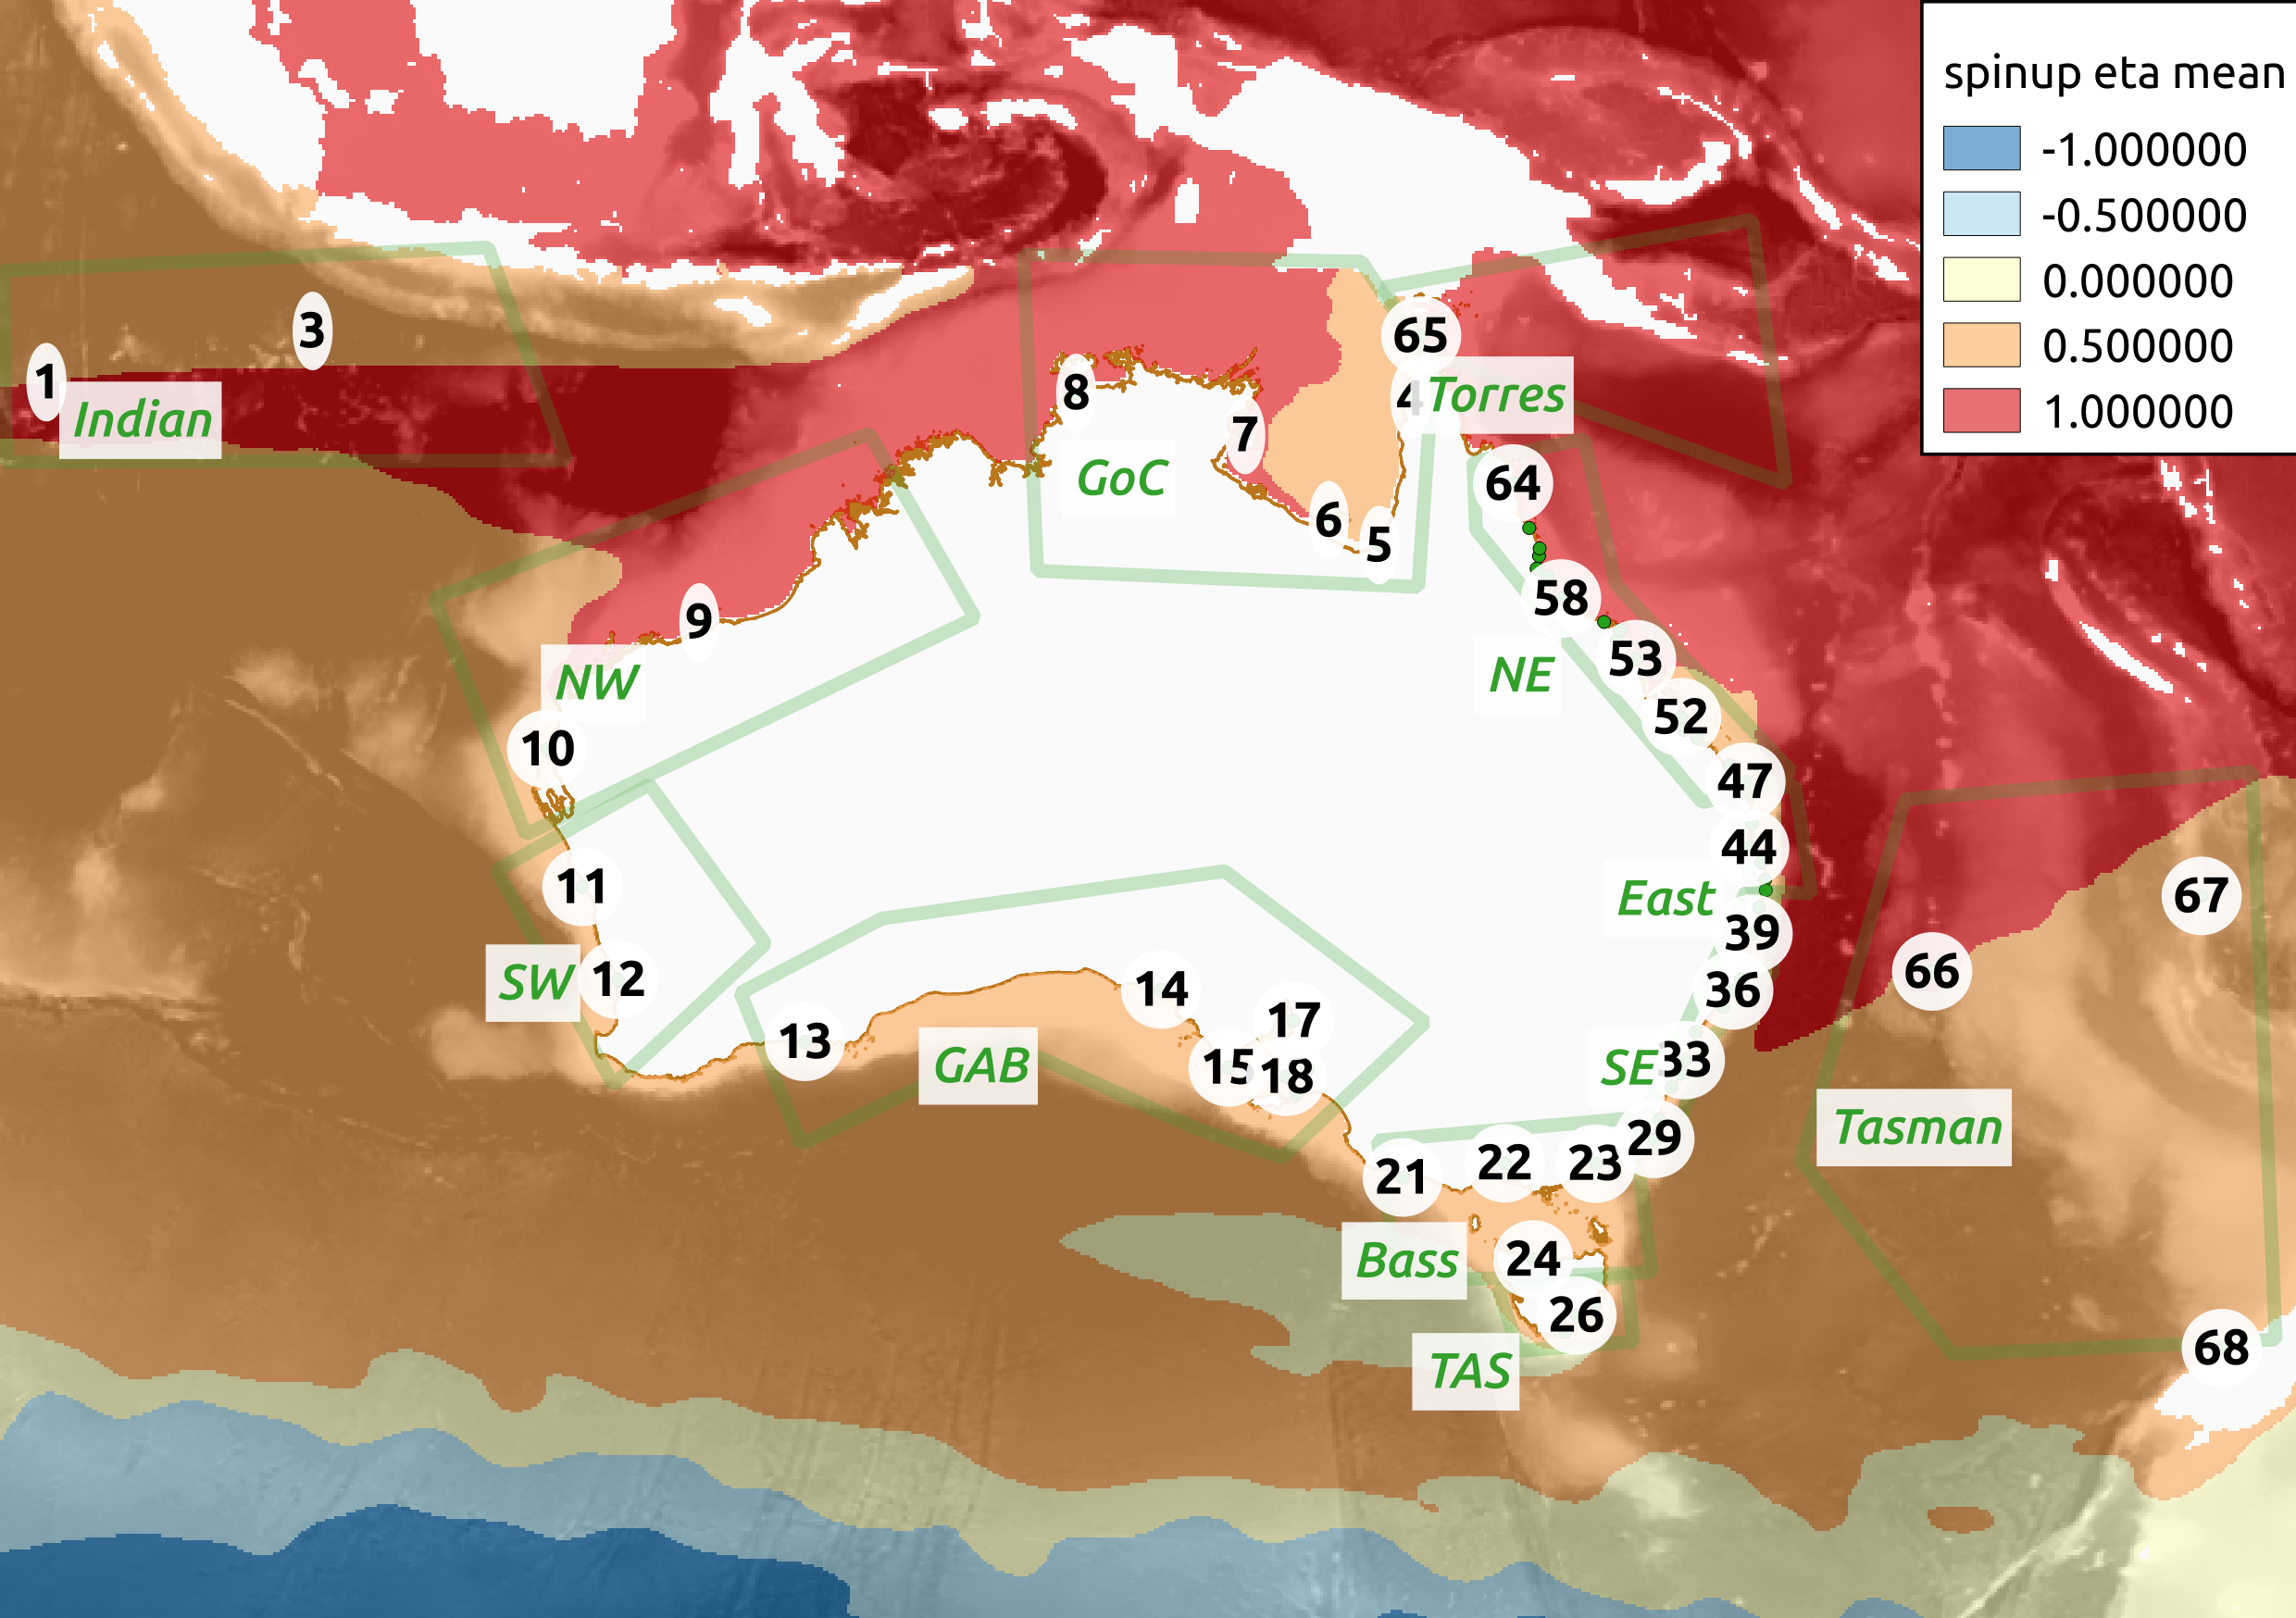
\includegraphics[width=1.0\textwidth]{figures/maps/omaps_bathy_and_eta.png}
    \caption{Geographic overview of evaluation sites in the Australia region.}
    {Ocean model bathymetry is indicated by grey background shading.  Colour contours illustrate the `spin up' model mean dynamic topography referenced below.  Tide gauge locations are identified with sequential numbers with order chosen to loosely align with anti-cyclonic coastal wave propagation direction. Regional groupings are referenced in subsequent results.}
    \label{fig:map_locations}
\end{figure}  

The observation locations are quite diverse with regard to exposure to the open ocean, instrumentation, sample frequency and communications quality. 


\subsection{Forecast goodness}
In general, forecast goodness cannot be properly judged against any single measure.
The~evaluation below is informed by the the concepts of `quality' and `value' following Murphy~\citep{Murphy:1993dh}.
Even if the component parts contain comparative technical deficiencies, the whole package may offer real value above available alternatives.
For this routine guidance use-case, only full time series statistics are presented as an evaluation. 
Categorical and event-based measures are not addressed in this paper.


Harmonic tide predictions considered in light of recent residuals commonly offer remarkably good guidance for coastal sea level.
Such a `tide + persisted residual' scheme is formulated in Equation~(\ref{eq:tide_res}) and taken as an appropriate benchmark against which to evaluate the aggregated forecast.
For~the new scheme to offer value at a particular location it must demonstrate superior skill relative to this~benchmark.  
\begin{equation}
h_{T+r}(t) = \eta_{T}(t) + r(t0)
\label{eq:tide_res}
\end{equation}

Following Equation (\ref{eq:aggSL}) where $r(t0)$ is the difference between observations and tide prediction $\eta_{T}$ at or just prior to forecast base time. 

\subsection{Highlighted behaviour}
The time series shown in Figure \ref{fig:ts_melb} is included as an example of a skilful dynamic model contribution.  
This location is subject to relatively powerful sea level variations associated with mid-latitude weather.
Of interest is the fact that the embayment in which the observations are taken is not represented at all in the ocean model.  This indicates the large influence of sea level outside of the bay at these timescales. 

\begin{figure}[!hbt] \centering
    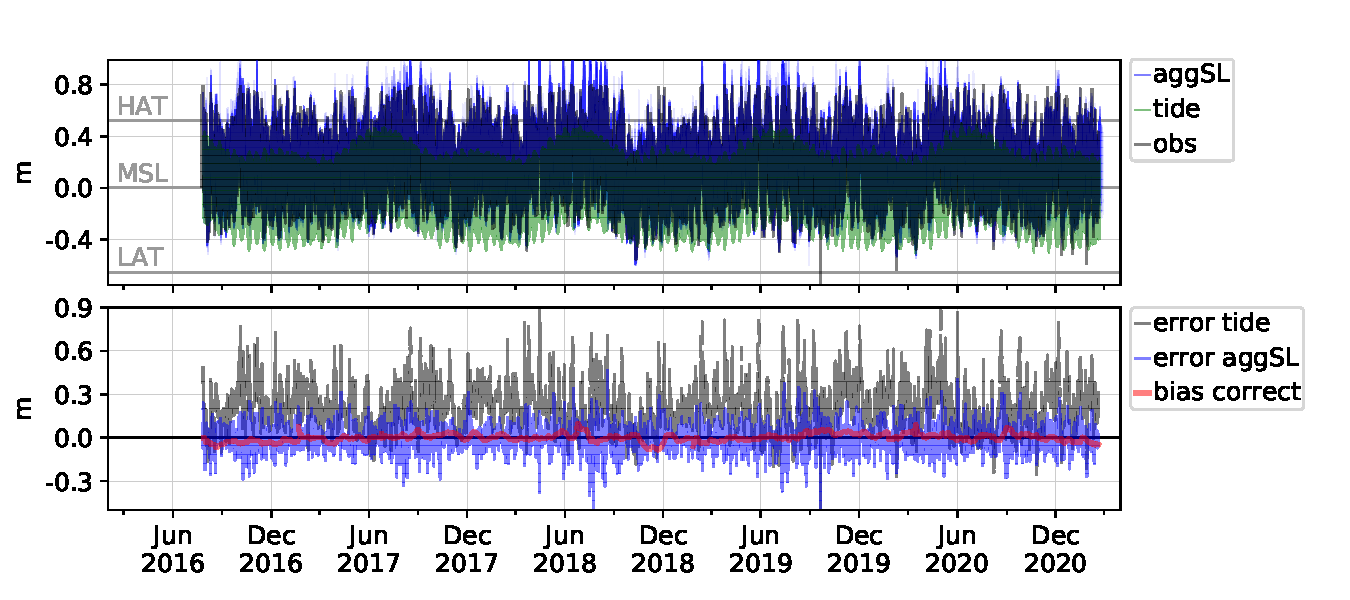
\includegraphics[width=\figwidthFull]{figures/plots/586204_verify_ts.pdf}
    \caption{Example time series at Melbourne.}
    {Location (\textbf{22} in Figure \ref{fig:map_locations} ); Upper panel shows total still water levels relative to conventional tidal benchmarks. Lower panel shows error signals and bias correction evolution.  Errors (residuals) are shown overlaid for standard tides and aggregate forecasts (`aggSL').  An~overall reduction in error variance is apparent between standard tides and aggregate forecasts.}
\label{fig:ts_melb}
\end{figure}   


Contrasting behaviour is illustrated in Figures \ref{fig:pdf} and \ref{fig:rms} by means of error statistics.
At all three locations the aggregated forecasts offer `quality' in the sense of matching observations; but for different reasons and different degress of potential value. 

\begin{figure}[!hbt] \centering
    \begin{subfigure}{0.30\textwidth}
    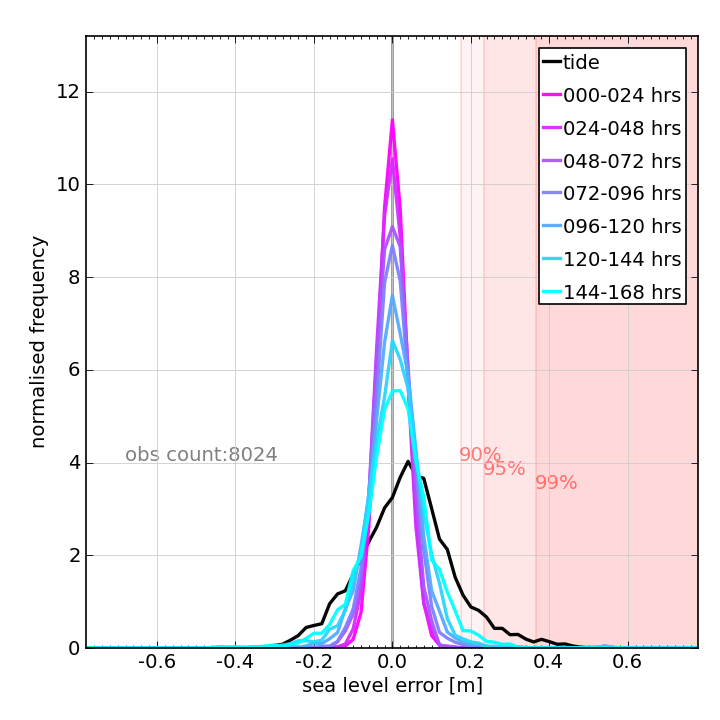
\includegraphics[width=0.9\textwidth]{figures/plots/0013_verify_pdf.png}
    \caption{}
    \end{subfigure}
    \begin{subfigure}{0.30\textwidth}
    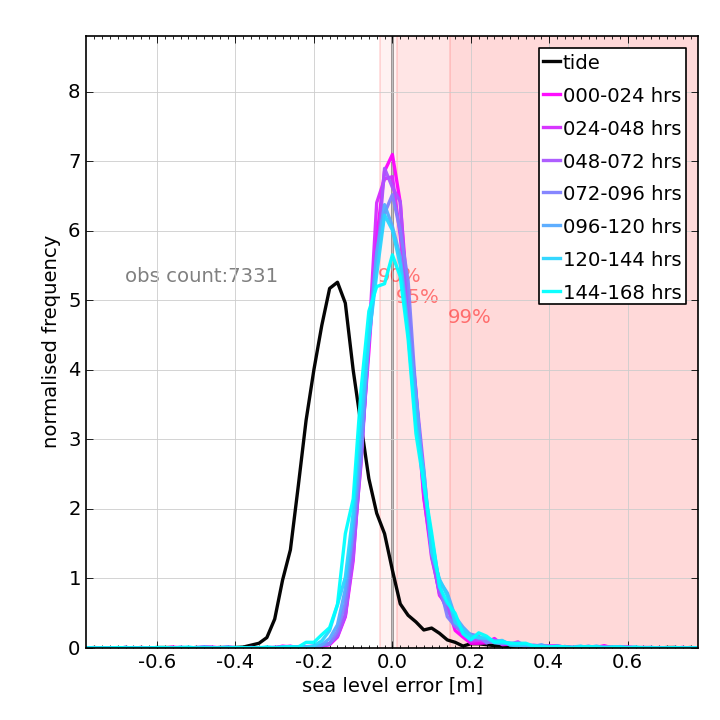
\includegraphics[width=0.9\textwidth]{figures/plots/0043_verify_pdf.png}
    \caption{}
    \end{subfigure}
    \begin{subfigure}{0.30\textwidth}
    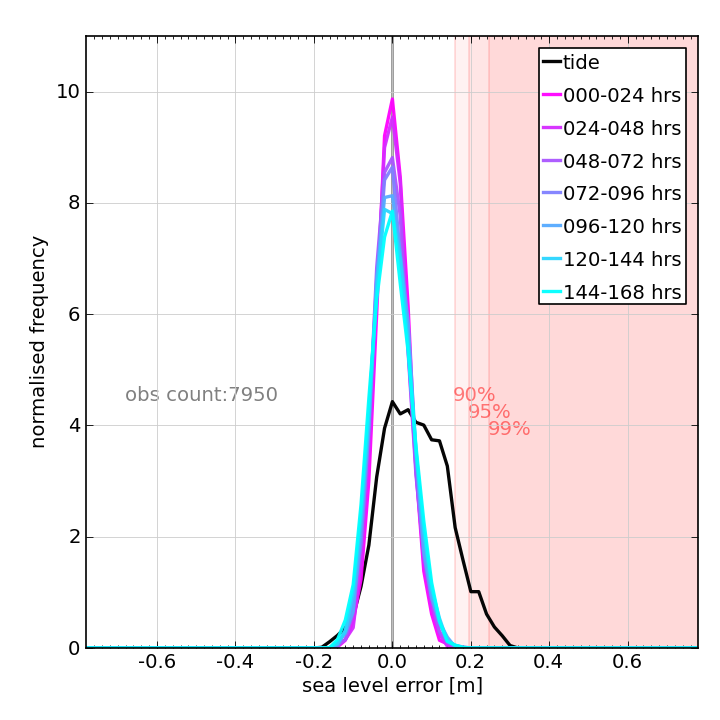
\includegraphics[width=0.9\textwidth]{figures/plots/0003_verify_pdf.png}
    \caption{}
    \end{subfigure}
    \caption{Forecast error distributions at selected locations.}
    {Skill improvement over standard harmonic tides is driven by different aspects of the generic aggregation process. (\textbf{a}) shows skill gain due to forecast signals associated with mid-latitudee weather (\textbf{b}) shows the practical problem of mismatched reference datums between real-time observational data and tide predictions (see Section~\ref{sec:bias_more}), (\textbf{c}) is a location at which longer period deviations from tide predictions are relatively powerful. (\textbf{a}) Site 13, Mid-latitude weather; (\textbf{b}) Site 43, Tide datum mismatch; (\textbf{c}) Site 3, Long period anomalies.}

    \label{fig:pdf}
\end{figure}   


\begin{figure}[!hbt] \centering
    \begin{subfigure}{0.30\textwidth}
    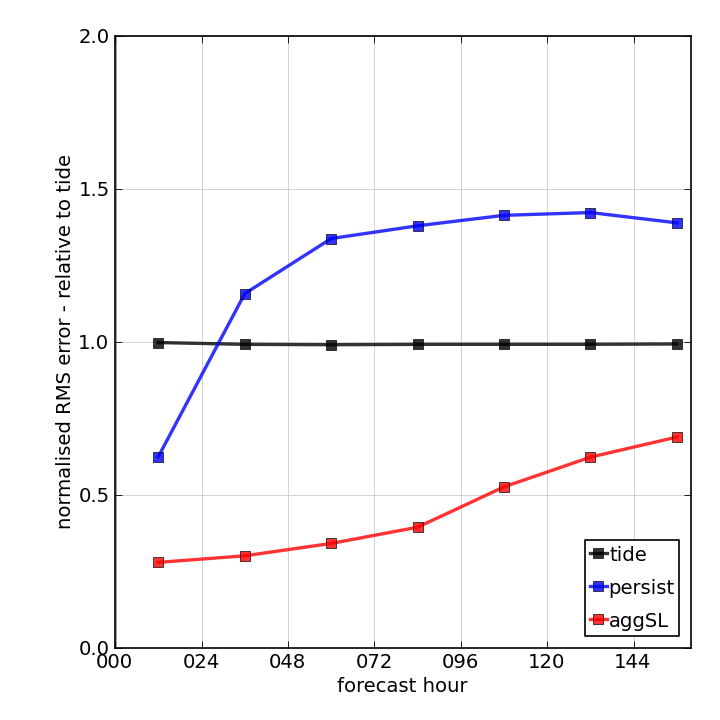
\includegraphics[width=0.9\textwidth]{figures/plots/0013_rms_growth.png}
    \caption{}
    \end{subfigure}
    \begin{subfigure}{0.30\textwidth}
    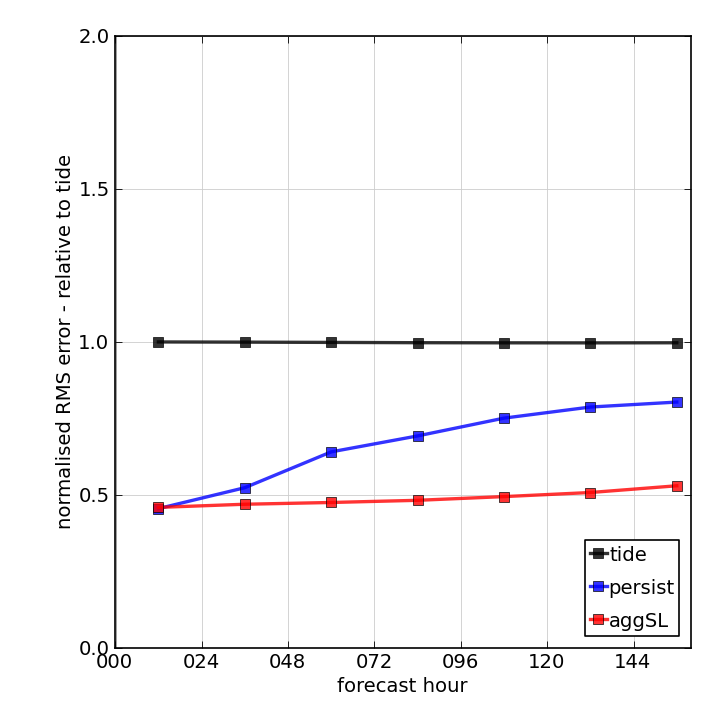
\includegraphics[width=0.9\textwidth]{figures/plots/0043_rms_growth.png}
    \caption{}
    \end{subfigure}
    \begin{subfigure}{0.30\textwidth}
    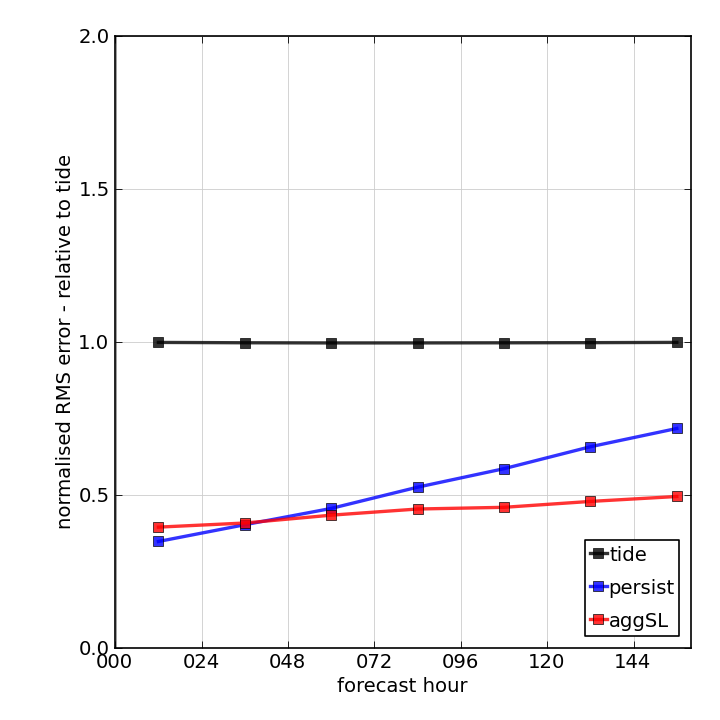
\includegraphics[width=0.9\textwidth]{figures/plots/0003_rms_growth.png}
    \caption{}
    \end{subfigure}
    
    \caption{Relative error metrics at selected locations.}
    {Following identical layout as Figure \ref{fig:pdf}. RMSE at increasing forecast lead times is normalised and plotted relative to the standard tidal residual---such that a lower value represents greater accuracy. Error growth with forecast age is evident. (\textbf{a}) As per (a) in Figure \ref{fig:pdf}; (\textbf{b}) As per (b) in Figure \ref{fig:pdf}; (\textbf{c}) As per (c) in Figure \ref{fig:pdf}.}
    \label{fig:rms}
\end{figure}   

\subsection{Skill summary: non-tidal information decay}
\label{sec:skill}

In order to highlight the differentiation between dynamic forecast skill between locations, Figure~\ref{fig:taylors} summarises average forecast evolution characteristics using Taylor diagrams \citep{Taylor:2000wp} for time series that have been de-tided using a band-limited harmonic tide.
Each `comet' contains a point for each 24~h period of the 7-day forecasts.
Site number is located at the 1st day forecast point.
Both the reference observations and forecasts have been de-tided using only the nominally gravitational tide signal described in Section \ref{sec:harmonics}.
All statistics are centred and normalised relative to the reference observation value $\hat{h}_{OBS}$ as defined in Equation (\ref{eq:taylor}).
\begin{equation}
\begin{split}
\hat{h}_{OBS}(t) &= h_{OBS}(t) - (\eta_{T}(t) - \eta_{HA}(t))  \\ 
\hat{h}_{FC}(t)  &= \eta_{SLA}(t) + \eta{LIB}(t) + b(t0) 
\label{eq:taylor}
\end{split}
\end{equation}

Following Equation (\ref {eq:aggSL}).  Where $\hat{h(t)}$ is sea level de-tided using a band-limited tidal time series.  

\begin{figure}[!hbt] \centering
    %------ 1
    \begin{subfigure}{0.30\textwidth}
        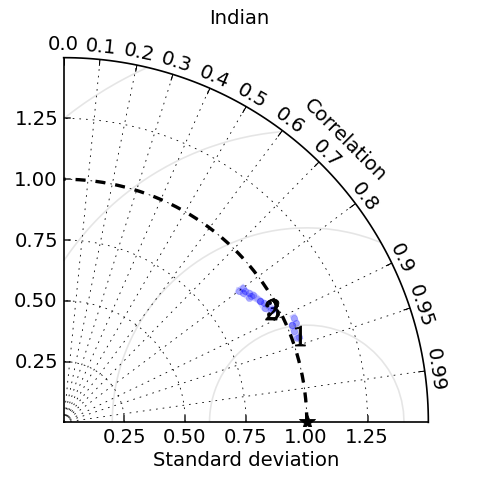
\includegraphics[width=\textwidth]{figures/plots/taylor_diag_res_Indian.png}
        \caption{}
    \end{subfigure}
    \begin{subfigure}{0.30\textwidth}
        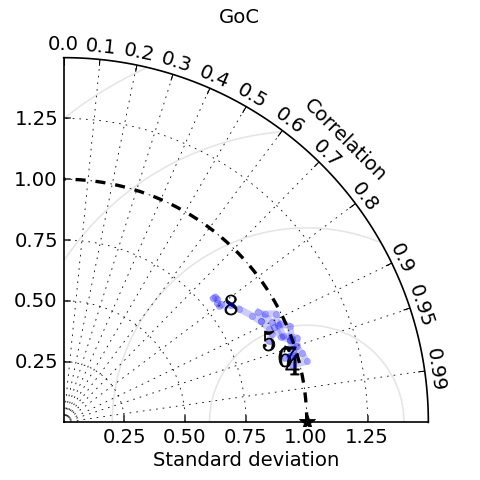
\includegraphics[width=\textwidth]{figures/plots/taylor_diag_res_GoC.png}
        \caption{}
    \end{subfigure}
    \begin{subfigure}{0.30\textwidth}
        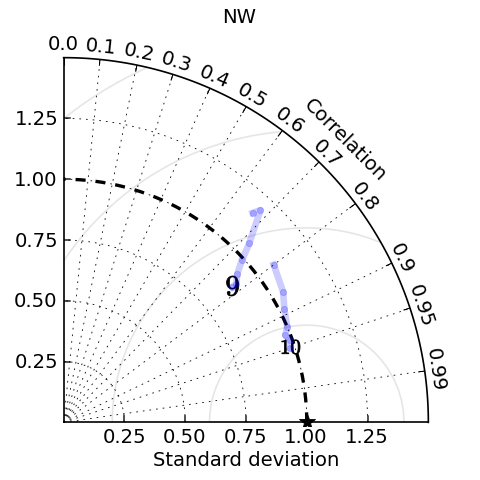
\includegraphics[width=\textwidth]{figures/plots/taylor_diag_res_NW.png}
        \caption{}
    \end{subfigure}
    %-------2
  \begin{subfigure}{0.30\textwidth}
     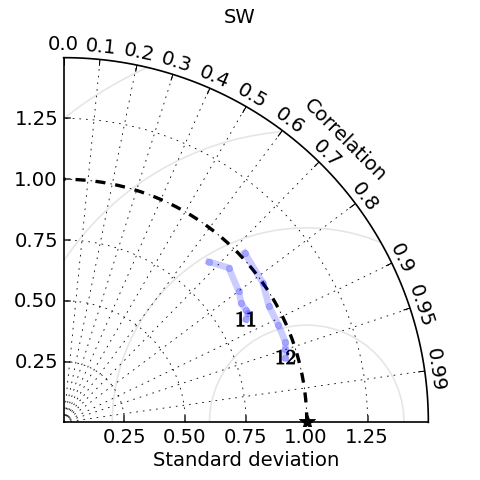
\includegraphics[width=\textwidth]{figures/plots/taylor_diag_res_SW.png}
        \caption{}
    \end{subfigure}
    \begin{subfigure}{0.30\textwidth}
        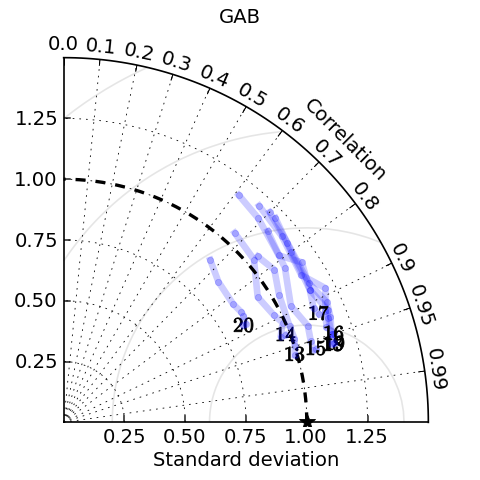
\includegraphics[width=\textwidth]{figures/plots/taylor_diag_res_GAB.png}
        \caption{}
    \end{subfigure}
    \begin{subfigure}{0.30\textwidth}

        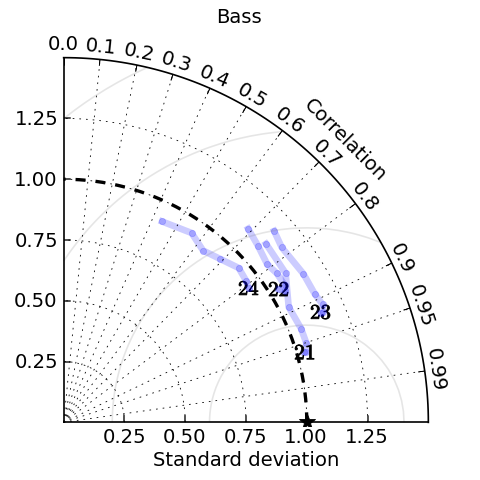
\includegraphics[width=\textwidth]{figures/plots/taylor_diag_res_Bass.png}
        \caption{}
    \end{subfigure}
    %-------3
    \begin{subfigure}{0.30\textwidth}
          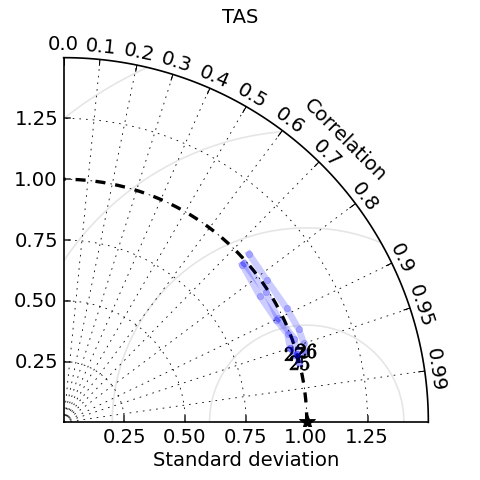
\includegraphics[width=\textwidth]{figures/plots/taylor_diag_res_TAS.png}
        \caption{}
    \end{subfigure}
    \begin{subfigure}{0.30\textwidth}
        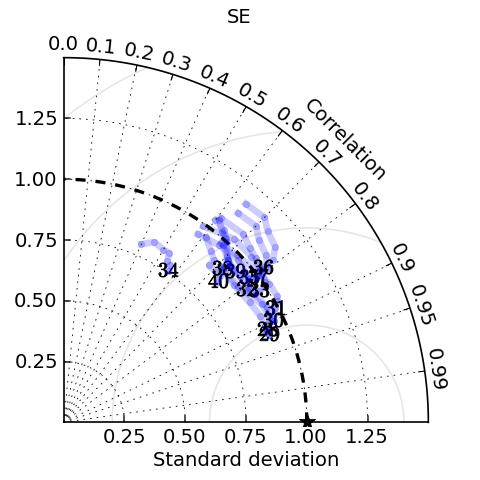
\includegraphics[width=\textwidth]{figures/plots/taylor_diag_res_SE.png}
        \caption{}
    \end{subfigure}
    \begin{subfigure}{0.30\textwidth}
        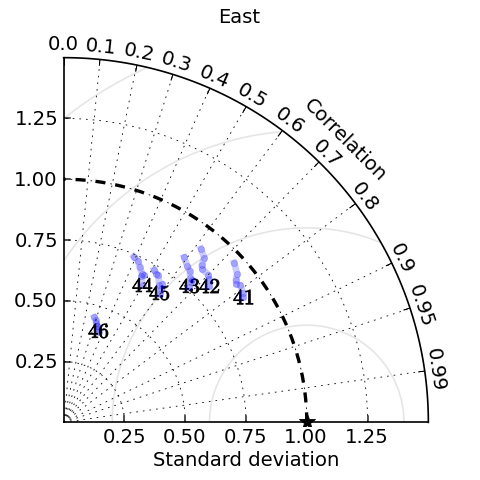
\includegraphics[width=\textwidth]{figures/plots/taylor_diag_res_East.png}
        \caption{}
    \end{subfigure}
    %-------4
    \begin{subfigure}{0.30\textwidth}
        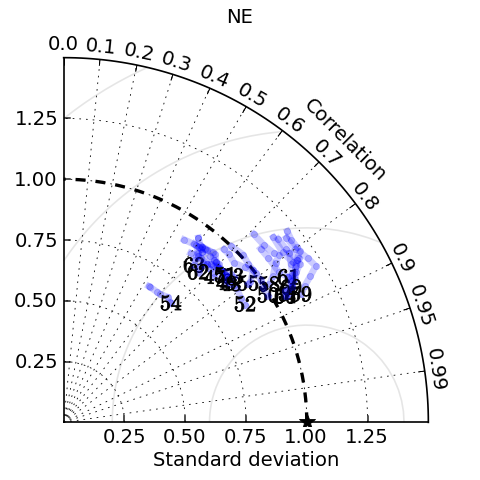
\includegraphics[width=\textwidth]{figures/plots/taylor_diag_res_NE.png}
        \caption{}
    \end{subfigure}
    \begin{subfigure}{0.30\textwidth}
        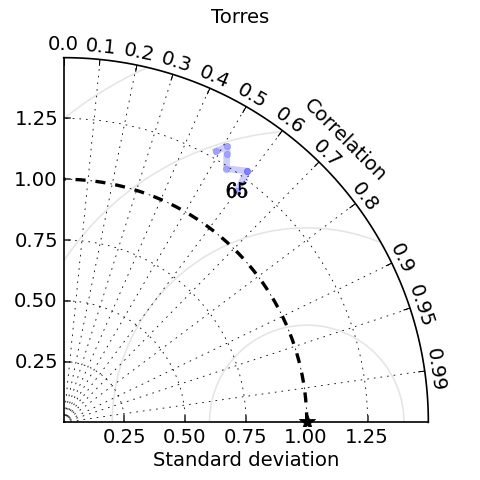
\includegraphics[width=\textwidth]{figures/plots/taylor_diag_res_Torres.png}
        \caption{}
    \end{subfigure}
    \begin{subfigure}{0.30\textwidth}
        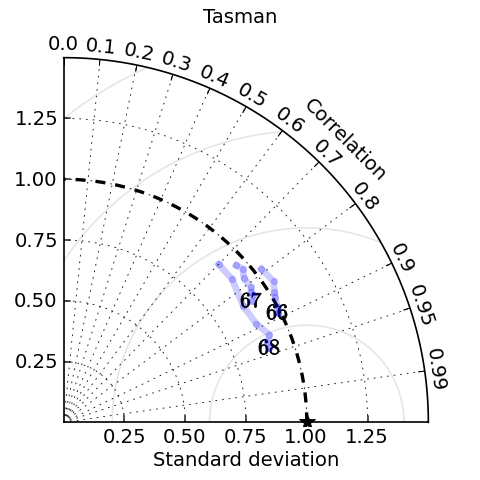
\includegraphics[width=\textwidth]{figures/plots/taylor_diag_res_Tasman.png}
        \caption{}
    \end{subfigure}
    %--------
    \caption{Taylor diagrams summarising skill evolution.}
    {Summary of dynamic skill evolution across 7-day forecasts where each `comet' describes average statistics for one location.
    Panels are divided according to regions shown in Figure~\ref{fig:map_locations}.
    Statistics are derived from filtered time series, not total sea level, and are normalised relative to the reference observations. (\textbf{a}) Indian; (\textbf{b}) Gulf of Carpentaria; (\textbf{c}) North West; (\textbf{d}) South West; (\textbf{e}) Great Aust Bight; (\textbf{f}) Bass Strait; (\textbf{g}) Tasmania; (\textbf{h}) South East; (\textbf{i}) East; (\textbf{j}) North East; (\textbf{k}) Torres Stait; (\textbf{l})~Tasman Sea. }
    \label{fig:taylors}
\end{figure}   
A notable feature of this visualisation is the decorrelation with forecast lead time.   
This is expected behaviour of a skilful deterministic forecast model where errors grow due to explicit numerical approximation of chaotic dynamics. 
Regional differences are apparent in degree of initial correlation and rate of decorrelation.

The under-prediction of variability in the `East' region (panel i) appears to reflect the noisy observational data streams from these 3rd party sites - such that the observation reference variability is inflated by communications glitches.

Anomalous variability growth for station 9 in `NW' region (panel c) was found to reflect the influence of a small number of over-forecast tropical cyclone events.  While the resolution limitations of the atmospheric forcing rule out applicability to extreme storm surge forecasts, NWP systems do evolve TCs that subsequently drive sea level signals in the OceanMAPS. In this case, the relative size of these over-forecasts at longer lead times is reflected in the Taylor diagram `comet'.

Torres Strait stands out for general poor performance and will be the subject of future~investigation.



\subsection{Skill summary: comparison against `tide + persisted residual'}
Based on the relative RMSE evaluation shown in Figure \ref{fig:rms} a traffic-light summary map of results is shown in Figure \ref{fig:map_rms}.
A red symbol indicates that aggregated forecast RMSE score is lower (better) than that of the reference `tide + persisted residual' for the specified forecast lead time, a blue symbol indicates the opposite.  Where neither is better than standard tides, a black symbol is allocated.   

\begin{figure}[!hbt] \centering
    \begin{subfigure}[b]{0.45\textwidth}
        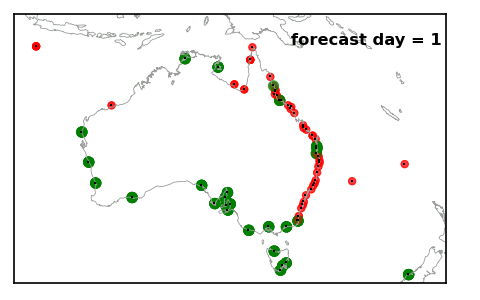
\includegraphics[width=\textwidth]{figures/maps/plot_map_rms_score_day_1.png}
    \end{subfigure}
    \begin{subfigure}[b]{0.45\textwidth}
        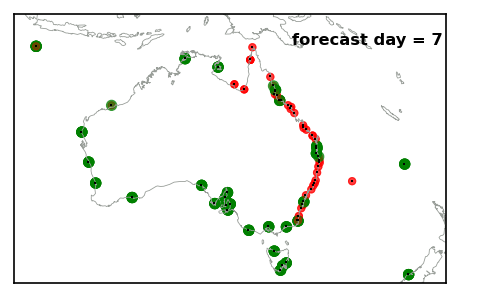
\includegraphics[width=\textwidth]{figures/maps/plot_map_rms_score_day_7.png}
    \end{subfigure}
    \caption{Summary map for RMS error reduction.}{Icons reflect which forecast source provides best information on average with regard to RMS error reduction. Red symbols at locations where aggregated forecast is best, blue for `tide + persisted residual' and black for standard tides.  Forecast lead times of 0--24 h are shown in left panel, and 144--168 h on the right.}
    \label{fig:map_rms}
\end{figure}   


%-------------------------------------------------------------------------
\section{Role of bias correction component}
\label{sec:bias_more}

The practical behaviour of the bias correction term is of special interest for evaluation.   
It is the only data driven term allowed to evolve in operations as described in Section \ref{sec:bias}.
An example time series is shown in the lower panel of Figure \ref{fig:ts_melb}.
The relatively static nature is typical of other sites.


To characterise behaviour each bias correction record was decomposed into a mean and temporarily varying signal.

%% mean
The mean bias correction is primarily aligned with the ocean model representation of mean dynamic topography MDT (compare \citep{Slobbe:wk}).
Such a reference surface in model space is the most common strategy used in the assimilation of altimetry observations, which are themselves constructed as anomalies from a reference surface in observation space. For OceanMAPS this surface was derived from a long free `spin up' run of the model \citep{Oke:2013fm}. 
Figure \ref{fig:bias_mean} shows the correspondence between model MDT ($\eta_{spinup}$) and the \textit{negative} of the bias correction mean.   The wider spatial distribution of MDT is indicated by contours in Figure \ref{fig:map_locations}.

\begin{figure}[!hbt] \centering
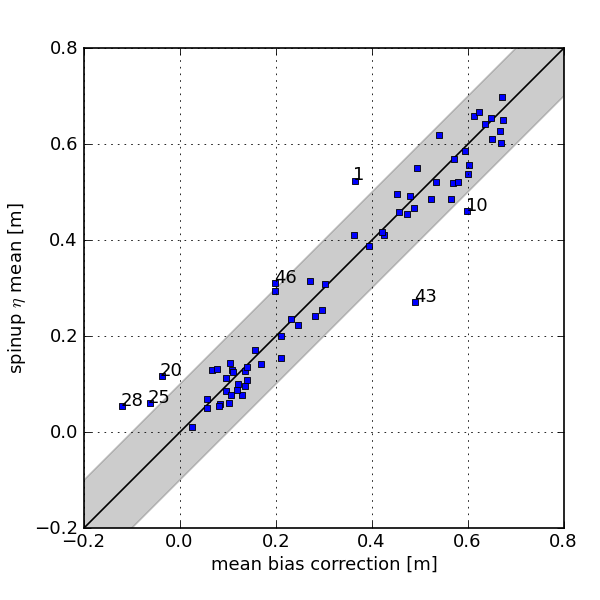
\includegraphics[width=0.5\textwidth]{figures/plots/aggSL_bias_breakdown_plot_1.png}
\caption{Mean bias correction versus model MDT surface.}{Magnitude of the temporal mean of bias correction history matched against model MDT surface at each location. An arbitrary mismatch threshold of 10 cm is used to highlight apparent outliers.}
\label{fig:bias_mean}
\end{figure}   

As the model MDT is known apriori, this correspondence supports the expectation that it is a~good first guess of the bias term.

Several sites deviate from this alignment by more than a fixed arbitrary threshold of 10 cm, and~these are distributed across the domain.
% This simple metric does not account for the wide range of signal variance around the coast. 
A large deviation indicates that the bias correction term systematically adjusted for information not available in the modelling systems alone.  


Site 46 is an esturine location where observations are strongly effected by surrounding sand sediment. The bias term at this location is partially adjusting to the asymmetry of the choked tidal~signal. 


Model sources of bias are feasible and likely.
However, of special note is the possibility of datum metadata mismatch between the available real-time observation data stream and the standard tide predictions. 
Site 43 is an example of a 3rd party datastream with such~a~mismatch. 

This is a symptom of organisational rather than modelling factors.   
Australian tide gauges are owned and operated by different bodies under a variety of data sharing arrangements.
Consistent metadata management from these diverse agencies remains problematic, despite being a nominally simple matter.

Tide predictions in Australia are reported relative to `prediction datum' which \textit{typically} aligns with the promulgated lowest astronomical tide (LAT) value.   
From time to time either the value for LAT or the alignment of prediction datum may be updated.  
% Real-time observations may have become available within the operational centre for reasons other than tide monitoring; in particular when such data is collated with river flood warning information.  
While overall the real-time data is expected to be reported relative to either instrument zero, Australian Height Datum (AHD) or tidal prediction datum, operational systems avaiable at the time of writing cannot reliably manage these differences.
% 1   200865   Cocos
% 10  6108     Cape Cuvier 
% 20  523757   Cape Jervis SA
% 25  94243    South port TAS
% 28  69129    TwoFold NSW
% 43  40881    AirSea at QLD << used in example
% 46  540311   Nooosa bar ... sedimentation within sand bar , low value clips


%% temporal
The temporally varying bias correction signals for each station are arranged in numbered order in Figure~\ref{fig:bias_time}.
Column order is such that adjacent stations are together, though separation distance varies greatly. 
In this visualisation it is apparent that the time varying signal has relatively small amplitude of~$<$7 cm for the majority of sites.
The single station located Torres Strait is a stand-out exception.  The~sea level signal at this location is the subject of further investigation, but for the present purpose will be disregarded as not valid.  


\begin{figure}[!hbt] \centering
    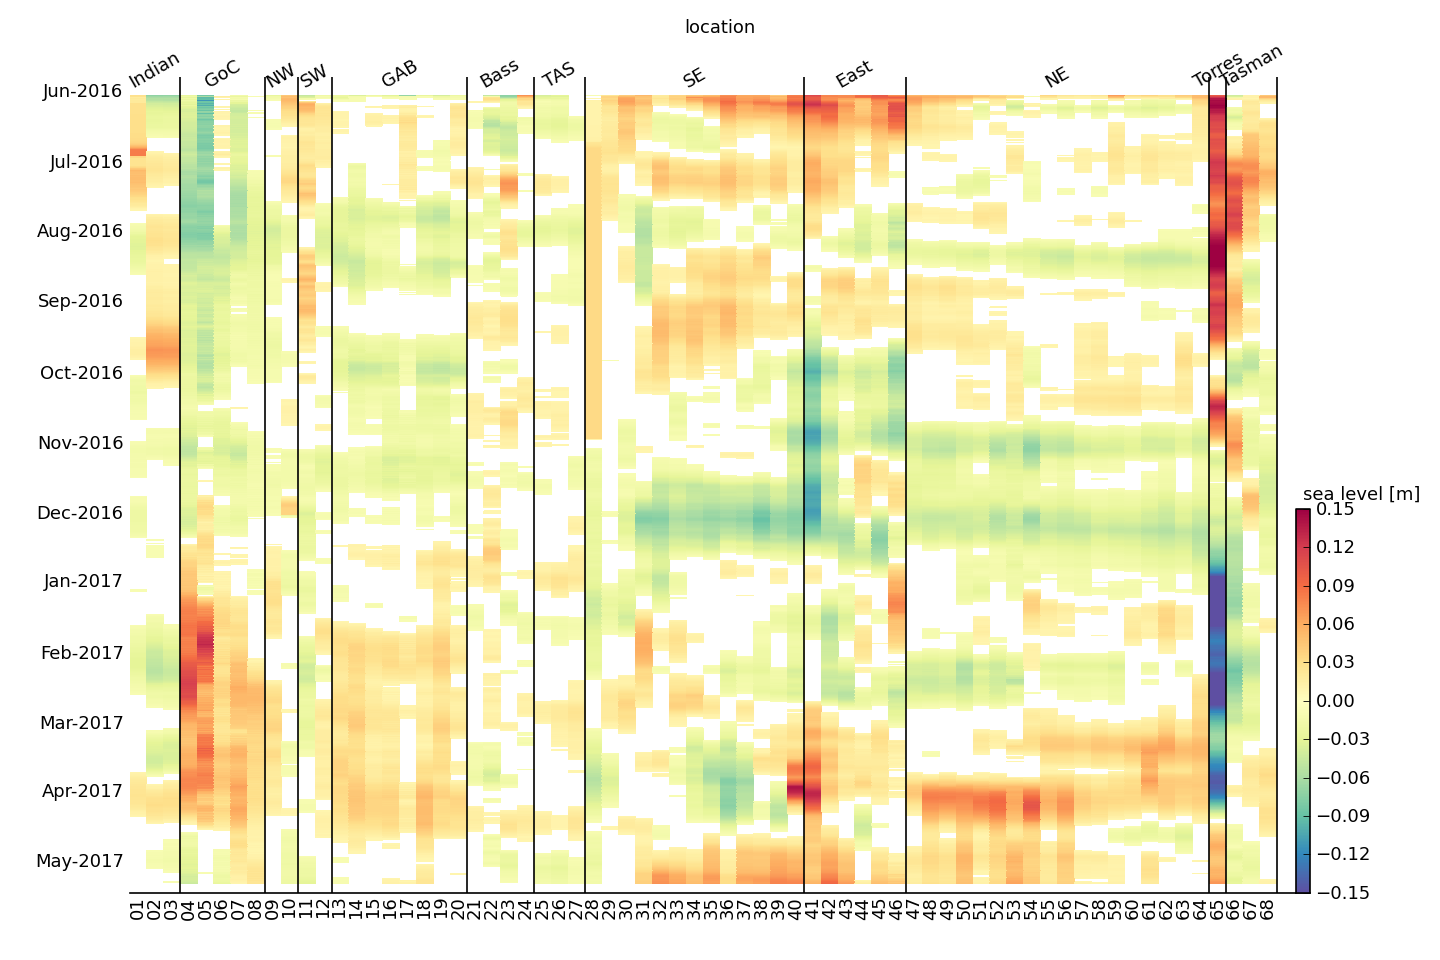
\includegraphics[width=1.0\textwidth]{figures/plots/aggSL_bias_breakdown_plot_2.png}
    \caption{Temporal signal from bias correction.}{The time-varying component of the bias correction signal after subtraction of respective mean offsets.  Absolute values less than 0.01 m are shown as white.  A degree of coherence is apparent between adjacent sites within the regional groupings-shown on map in Figure \ref{fig:map_locations}. } 
\label{fig:bias_time}
\end{figure}  


%%%%%%%%%%%%%%%%%%%%%%%%%%%%%%%%%%%%%%%%%%
\section{Chapter discussion}
\subsection{Adequacy and value}
The aggregation method offers generally improved sea level forecasts by drawing a pragmatic balance between the strengths of existing operational systems.
A common configuration for all sites was employed for robustness and to facilitate expansion to new locations.  
Although real-time observations are exploited when available, the simple bias correction scheme is relatively robust to data gaps and noise. 
The balance of contributions from component terms varies with timescale and location around the Australian coast.
Regional groupings are apparent in the skill characteristics of the forecasts.
By producing a quantity that can be directly compared to observations and reference tidal planes, forecasts can be presented intuitively along with recent real-time sea level and provide ongoing and immediate verification---as is Figure \ref{fig:fc_eg}.

The skill level and value offered by these forecasts sets a benchmark against which any new sea-level forecasting capabilities can be compared and contrasted.  

\subsection{Spatial interpolation}
The characteristics demonstrated by the bias correction scheme indicate that meaningful forecasts may be produced at intermediate sites at which real-time observations are not available.
The patterns of regional coherence indicate that spatial interpolation of bias correction values may be worthy of further investigation.
Figure \ref{fig:bias_time} indicates that spatial interpolation within regions `GAB' and `NE' is particularly promising.

Appropriate consideration of geography and other factors on validity will be required.
Strongly contrasting bias correction characteristics at Torres Strait (site 65) highlight the importance of not ignoring geography.

While the irregular spatial sampling across the domain is undesirable, there is real prospect to obtain access to many more tide gauges that are known to exist but not report real time data to the BoM.   
Such additional locations will facilitate future investigation of spatial interpolation approaches.    


\subsection{Extensions}
The aggregation concept presented is flexible.
It is foreseeable that additional or alternative operational inputs could be incorporated. 
The potential to seamlessly include short-range higher resolution forecast information, while maintaining the 7-day outlook, is a logical extension given the aim of exploiting existing capabilities.
On the other hand, NWP forecasts currently cover out to 10-days lead time. The option of extending the length of ocean forecasts to match is worthy of consideration in light of this sea level evaluation (such as in Figure \ref{fig:rms}).

Uncertainty information can already be roughly indicated by means of presenting overlaid sequential forecasts as in Figure \ref{fig:fc_eg}.
Optimal treatment of the lagged ensemble and communicating error growth to users is an outstanding need.
Developments in ensemble NWP systems within the operational centre are expected to provide additional sampling of uncertainty and enable further development of this important aspect of sea level forecasts.  

